\documentclass[11pt,a4paper]{article}
\usepackage[margin=2.2cm]{geometry}
\usepackage{graphicx,booktabs,amsmath,xcolor,float}
\usepackage[hidelinks]{hyperref}
\usepackage[font=small,labelfont=bf]{caption}
\newcommand{\pc}{p_c}
\title{The audiovisual bias: measure it in a cross-modal block,\\ or leave it out of the bimodal fits?}
\author{av-dur v2 \quad 30 October 2026}
\date{}
\begin{document}
\maketitle
\vspace{-1.5em}

\section*{Summary}
\textbf{Bottom line: ignoring the bias ($c = d = 0$) is a reasonable choice for the model comparison.} A cross-modal block does not help find the right model, even when its estimates are exact. It helps only the precision of $\pc$, it does so only with three standards, and only if the bias it measures carries over to the combined stimulus, which cannot be checked.
\begin{enumerate}
\item \textbf{Model recovery is the same with or without the bias.}
  \begin{itemize}
  \item Ignoring the bias finds the right model for 88.5\% of simulated participants.
  \item Plugging in the \emph{true} $c$ and $d$ also gives 88.5\% (paired difference 0.0 points, 95\% CI $-4.6$ to $+4.6$).
  \item The three-standard cross-modal block gives 88.5\% and the 500\,ms block 89.5\%.
  \end{itemize}
  This holds with $c$ spread twice as wide as in the earlier report (SD 0.23--0.26, as in v1) and $d$ as in the pilot (SD 0.19).
\item \textbf{Fitting $d$ freely is the worst option.} Model recovery falls to 82.2\% ($-6.3$ points, CI $-11.7$ to $-0.9$), and fusion is recognised in only 62\% of cases instead of 79\%. Do not use a free $d$ as the sensitivity check: it changes the winning model when nothing is wrong. In v1 (with $c$ fixed at the cross-modal value) it changed the winner for 2 of 11 participants with $\sigma_A$ tied and for 6 of 11 with $\sigma_A$ free.
\item \textbf{$\pc$ is where a cross-modal block helps,} for the 64 causal-inference participants:
  \begin{itemize}
  \item With three standards, if the bias transfers, the RMSE of $\pc$ falls from 0.184 to 0.135. Knowing the true bias gives 0.142. The paired change in absolute error is $-0.029$ (CI $-0.051$ to $-0.006$).
  \item The 500\,ms block alone gives 0.158; its paired change is not significant.
  \item If the bias does not transfer, there is no gain: 0.193 with fixed values, 0.176 with priors.
  \end{itemize}
\item \textbf{The bimodal data say little about the bias.} For the median participant, the true bias improves the generating model's fit by only about 1 AIC point. It is more than 10 points for 8\%.
\item \textbf{The v1 data agree.} With $\sigma_A$ tied to the unimodal block, fixing $c$ at each participant's cross-modal value left the winning model unchanged for 9 of 11, improved the summed AIC by only 10 points, and changed $\pc$ by at most 0.10.
\item \textbf{The cross-modal block itself works well.} It measures $c$ with an RMSE of 0.05--0.10 and $d$ with 0.11 (three standards). The problem is not its precision: the bias matters little for the bimodal fits.
\end{enumerate}

\paragraph{Recommendation.}
\begin{itemize}
\item \textbf{Main analysis:} $c = d = 0$, $\sigma_A$ and $\sigma_V$ tied to the unimodal blocks, AIC. State in the paper that the bias was not modelled, and cite these simulations and the v1 check.
\item \textbf{Add the three-standard cross-modal block} (744 trials, about 40--45\,min) only if precise per-participant $\pc$ values are part of the conclusions. Even then, the gain rests on the untestable assumption that the bias transfers. The 500\,ms block alone (about 25\,min) is not worth it.
\item \textbf{Drop ``$d$ free'' as the sensitivity check.} A check with $d$ fixed at a group value (e.g.\ the pilot's 0.25) would be cheap, but it was not simulated here.
\item \textbf{The pilot's three participants} with three standards can describe the bias itself in the paper, if a reviewer asks.
\end{itemize}

\section{The question}\label{sec:question}
The bias model is $\ln \hat v = \ln v - c_\text{noise} - d \ln(v / 0.5\,\text{s})$, applied to the visual measurement in both intervals. Here $c > 0$ means vision seems shorter than sound, and $d > 0$ means the bias grows with duration. Measured values:
\begin{itemize}
\item \textbf{v1:} cross-modal block at 500\,ms only, 11 participants. $c_\text{low}$ had a mean of 0.26 (SD 0.26) and $c_\text{high}$ a mean of 0.17 (SD 0.33), from $-0.25$ to $+0.84$. The two noise levels correlate at 0.79.
\item \textbf{v2 pilot:} 300, 500 and 800\,ms standards, P101, P102 and P104. $c$ ranged from 0.06 to 0.54. $d$ ranged from $-0.14$ to 0.63, with SEs of 0.09--0.26 per noise level.
\end{itemize}

The earlier report (\texttt{bias\_report.pdf}) showed that the main experiment cannot measure $c$. Under fusion $c$ cancels; under causal inference and switching it acts only through the perceived discrepancy. $d$ is measurable only for fusion observers whose $\sigma$s are known very precisely. Fitting $c$ and $d$ freely made model selection worse. What was never simulated is the alternative: \emph{measure $c$ and $d$ in a separate cross-modal block and give them to the bimodal fit.} This report compares that with ignoring the bias, on the same simulated participants:
\begin{center}
\begin{tabular}{lp{10.6cm}}
\toprule
fit & bias in the bimodal fit \\
\midrule
ignore & $c = d = 0$ (the current plan) \\
$d$ free & $c = 0$, $d$ fitted (the current plan's sensitivity check) \\
500\,ms block & $c$ fixed at the cross-modal estimates, $d = 0$ \\
3 standards & $c$ and $d$ fixed at the cross-modal estimates \\
3 standards, priors & $c$ and $d$ fitted, with Gaussian priors from the cross-modal estimates (roughly a joint fit) \\
true $c$, $d$ & fixed at the true values: the most any cross-modal block could give \\
\bottomrule
\end{tabular}
\end{center}
Each cross-modal option is run twice. In the first case the bias it measures is the bias in the bimodal trials (\emph{transfers}). In the second it is an unrelated value (\emph{no transfer}). The second case is your concern of 27 October: the bias of separate cues may not carry over to the combined stimulus.

\section{What was simulated}\label{sec:sim}
The code is listed under Files at the end.
\begin{itemize}
\item \textbf{Participants.} 191 simulated participants: 64 causal inference (CI), 63 forced fusion, 64 switching. 600 were planned; the run stopped at its 6.5-hour limit, with 10--21\,min of fitting per participant. Model parameters are drawn as in the earlier reports: $\lambda \sim U(0.001, 0.1)$, $\sigma_{A,\text{low}} \sim U(0.12, 0.45)$, $\sigma_{A,\text{high}} \sim U(0.55, 1)$, unimodal $\sigma_V \sim U(0.3, 1)$, $\pc$ and $p_\text{switch} \sim U(0.1, 0.9)$.
\item \textbf{Bias, from the measured values:}
  \begin{itemize}
  \item $c_\text{low} \sim N(0.26, 0.26)$ and $c_\text{high} \sim N(0.17, 0.30)$, correlated 0.8, as in v1.
  \item $d \sim N(0.25, 0.20)$: the v2 pilot's spread, once its estimation error is removed.
  \item Values are kept within $c \in [-0.5, 1]$ and $d \in [-0.3, 0.7]$.
  \item Drawn: $c_\text{low}$ mean 0.24 (SD 0.23), $c_\text{high}$ 0.14 (0.26), $d$ 0.25 (0.19).
  \end{itemize}
  This is about twice as wide as the earlier report's $c$ ($U(0, 0.5)$, SD 0.14). Ignoring the bias is therefore tested harder here than before.
\item \textbf{Main experiment as it now runs (from 29 Oct):}
  \begin{itemize}
  \item 9 conflicts ($\pm$450\,ms) $\times$ 2 noise levels.
  \item Per condition, a 2D1U and a 1D2U staircase of 50 trials each, plus 10 easy trials: 110 per condition, 1980 in all.
  \item Whole frames at 120\,Hz.
  \end{itemize}
\item \textbf{Unimodal blocks (150 + 20 QUEST+ trials each).}
  \begin{itemize}
  \item $\sigma_A$ is tied to its unimodal estimate (log error 0.2) by a Gaussian penalty on $\ln \sigma_A$.
  \item The unimodal visual $\sigma$ is measured with log error 0.2. It equals $\sigma_V / (1 - d)$, so the bimodal $\sigma_V$ is that value $\times (1 - d)$, with $d$ the value the fit uses.
  \end{itemize}
\item \textbf{Cross-modal block, as it ran:} an auditory test against a visual standard, at both noise levels.
  \begin{itemize}
  \item 500\,ms: a 1D1U pair, 2D1U and 1D2U, 45 trials each, plus 20 easy trials per noise level. 400 trials.
  \item 300 and 800\,ms: a 1D1U pair of 40 trials each, plus 6 easy trials per noise level. 172 trials each.
  \item The answers come from the same measurements as in the main experiment, plus the lapse:
  \[ P(\text{sound longer}) = \Phi\!\left(\frac{\ln a - m_v}{\sqrt{\sigma_A^2 + \sigma_V^2}}\right), \qquad m_v = (1-d)\ln v + d \ln 0.5 - c_\text{noise}. \]
  \item Fitted by maximum likelihood, with one lapse and a slope per noise level. The 500\,ms block alone gives $c_\text{low}$ and $c_\text{high}$; all three blocks give $c$ and $d$. SEs come from the Hessian, inflated by 1.2 because in a check of 60 simulated blocks they were 2--26\% too small.
  \end{itemize}
\item \textbf{No transfer:} the cross-modal block is simulated with an independent draw of $c$ and $d$ from the same distribution.
\item \textbf{Fits:} BADS, for each model and variant.
  \begin{itemize}
  \item Fusion is fitted first, and CI also starts from its solution with $\pc$ near 1, so CI never fits worse than fusion.
  \item Every variant except ``ignore'' also starts from the same model's ``ignore'' fit.
  \item Models are compared by AIC within each variant.
  \end{itemize}
\end{itemize}
Comparisons between fits are paired: the same participants and the same data. The 95\% CIs come from the per-participant differences. With 191 participants, a single recovery rate has a standard error of about 2.3 points overall and 4--5 points per generating model. Eight variants are compared with ``ignore'', so one CI excluding 0 by a small margin is expected by chance.

\section{Results}\label{sec:results}

\subsection{What the cross-modal block measures}
Table~\ref{tab:xm} and Fig.~\ref{fig:xm}. The block measures the bias well:
\begin{itemize}
\item $c$ with an RMSE of 0.05--0.10 against a true SD of 0.23--0.26 ($r \ge 0.93$);
\item $d$ with 0.11 against 0.19 ($r = 0.85$).
\end{itemize}
The intervals cover the true values 96--98\% of the time. Whatever follows is therefore not a problem of measurement precision.

\begin{table}[H]\centering\small
\begin{tabular}{llcccc}
\toprule
block & parameter & RMSE & $r$ & true SD & coverage of $\pm 1.96 \times 1.2$\,SE \\
\midrule
500\,ms & $c_\text{low}$ & 0.065 & 0.97 & 0.23 & 96\% \\
 & $c_\text{high}$ & 0.103 & 0.93 & 0.26 & 97\% \\
300 + 500 + 800\,ms & $c_\text{low}$ & 0.047 & 0.98 & 0.23 & 97\% \\
 & $c_\text{high}$ & 0.066 & 0.97 & 0.26 & 98\% \\
 & $d$ & 0.110 & 0.85 & 0.19 & 98\% \\
\bottomrule
\end{tabular}
\caption{Cross-modal estimates against the true bias (191 participants, bias transfers).}\label{tab:xm}
\end{table}

\begin{figure}[H]\centering
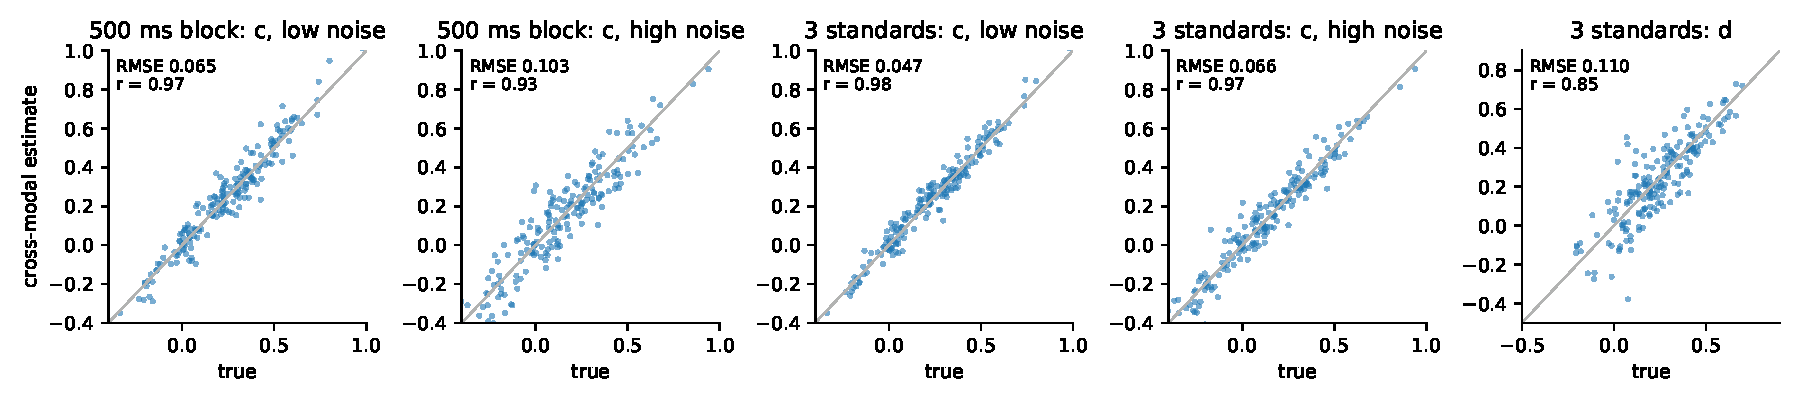
\includegraphics[width=\textwidth]{xm_crossmodal.pdf}
\caption{Cross-modal estimates against the true values. The 500\,ms block has no $d$ panel: with one standard, $\ln(v/0.5) = 0$, so $d$ drops out of its predictions and cannot be estimated; it is set to 0 there.}\label{fig:xm}
\end{figure}

\subsection{Model recovery}
Table~\ref{tab:rec}, Figs.~\ref{fig:rec} and~\ref{fig:conf}.
\begin{itemize}
\item \textbf{Knowing the bias does not help model selection.} With the true $c$ and $d$, recovery is 88.5\%, the same as when the bias is ignored. CI participants gain (86\% $\to$ 91\%), but more fusion participants are taken for CI (16\% $\to$ 22\%), and the two cancel. The cross-modal estimates do the same as the truth.
\item \textbf{The remaining errors are fusion participants taken for CI,} in every variant. CI contains fusion ($\pc = 1$), and AIC's 2-point penalty does not always stop CI from fitting noise. This is a property of the models, not of the bias.
\item \textbf{The 500\,ms block, ``no transfer'', looks best (91.1\%).} The reason is not a real benefit. A wrong $c$ makes CI fit slightly worse, while fusion is unaffected because $c$ cancels in it, so fewer fusion participants are taken for CI. Its CI only just excludes 0, among eight comparisons.
\item \textbf{$d$ free and the priors lose recovery,} mostly for fusion (62\% and 65\%). Each adds flexibility that CI uses more than fusion does.
\end{itemize}

\begin{table}[H]\centering\small
\begin{tabular}{lccccc}
\toprule
fit & all & CI & fusion & switching & difference from ignore (95\% CI) \\
\midrule
ignore ($c = d = 0$) & 88.5 & 85.9 & 79.4 & 100.0 & \\
$d$ free, $c = 0$ & 82.2 & 89.1 & 61.9 & 95.3 & $-6.3$ ($-11.7$, $-0.9$) \\
500\,ms block, $c$ fixed & 89.5 & 87.5 & 82.5 & 98.4 & $+1.0$ ($-1.5$, $+3.6$) \\
3 standards, $c$, $d$ fixed & 88.5 & 92.2 & 74.6 & 98.4 & $0.0$ ($-4.4$, $+4.4$) \\
3 standards, priors & 84.8 & 90.6 & 65.1 & 98.4 & $-3.7$ ($-8.8$, $+1.5$) \\
500\,ms block, no transfer & 91.1 & 89.1 & 84.1 & 100.0 & $+2.6$ ($+0.3$, $+4.9$) \\
3 standards fixed, no transfer & 86.4 & 84.4 & 74.6 & 100.0 & $-2.1$ ($-6.7$, $+2.5$) \\
3 standards priors, no transfer & 85.9 & 87.5 & 69.8 & 100.0 & $-2.6$ ($-7.5$, $+2.3$) \\
true $c$, $d$ & 88.5 & 90.6 & 76.2 & 98.4 & $0.0$ ($-4.6$, $+4.6$) \\
\bottomrule
\end{tabular}
\caption{Right model (AIC), \%, by generating model. Differences are paired, in percentage points.}\label{tab:rec}
\end{table}

\begin{figure}[H]\centering
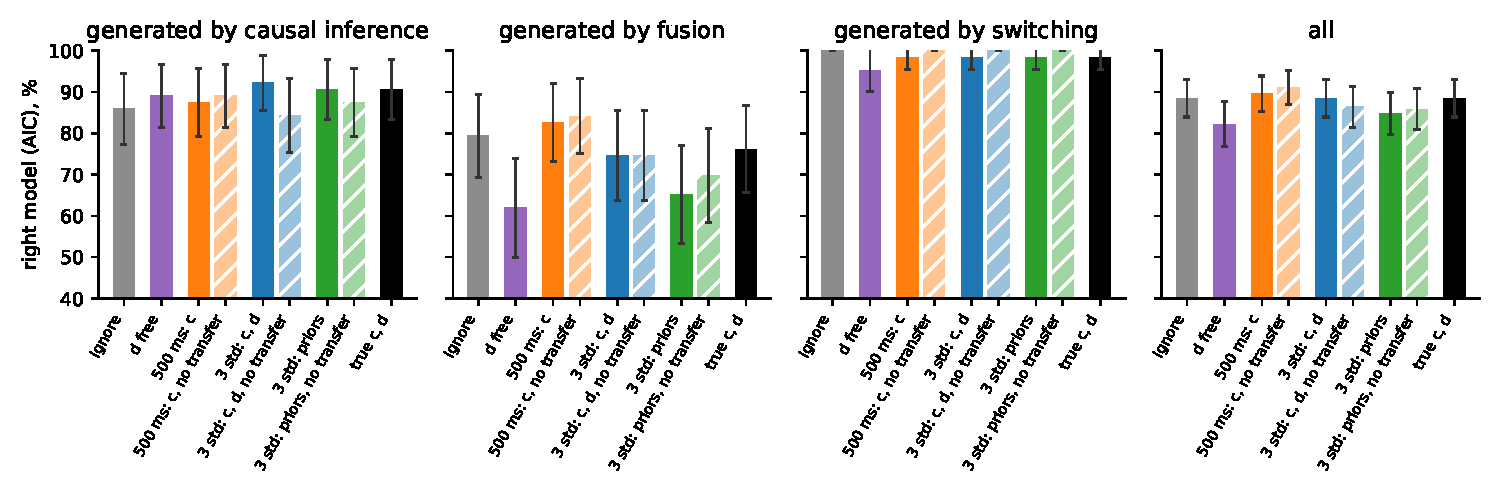
\includegraphics[width=\textwidth]{xm_modelrec.pdf}
\caption{Right model (AIC) by fit and generating model, with 95\% CIs. Hatched: the cross-modal bias does not transfer to the bimodal trials. Chance is 33\%.}\label{fig:rec}
\end{figure}

\begin{figure}[H]\centering
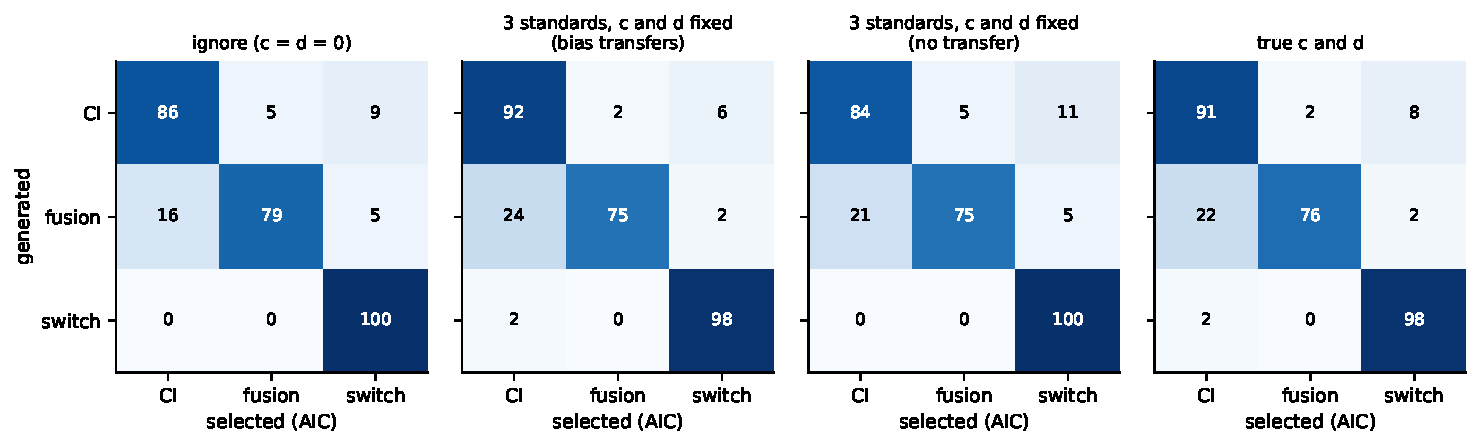
\includegraphics[width=\textwidth]{xm_confusion.pdf}
\caption{Selected model by generating model, \% of each row.}\label{fig:conf}
\end{figure}

\subsection{$\pc$ and $p_\text{switch}$}
Table~\ref{tab:pc} and Fig.~\ref{fig:pc}.
\begin{itemize}
\item \textbf{$\pc$} (64 CI participants, CI fit):
  \begin{itemize}
  \item With the bias ignored, $\pc$ is nearly unbiased (mean error $-0.01$), but its RMSE is 0.184.
  \item The three-standard block brings it to 0.135 if the bias transfers, as good as the true bias (0.142).
  \item The share of participants with $\pc$ off by more than 0.2 falls from 16\% to 12\%.
  \item The 500\,ms block gives 0.158, a change that is not significant.
  \item Without transfer, every cross-modal option is at least as bad as ignoring.
  \end{itemize}
\item \textbf{$p_\text{switch}$} is recovered well in every variant (RMSE 0.066--0.077).
\end{itemize}

\begin{table}[H]\centering\small
\begin{tabular}{lccccc}
\toprule
fit & \multicolumn{4}{c}{$\pc$ (CI participants)} & $p_\text{switch}$ \\
 & RMSE & $r$ & mean error & change in $|$error$|$ (95\% CI) & RMSE \\
\midrule
ignore ($c = d = 0$) & 0.184 & 0.69 & $-0.008$ & & 0.077 \\
$d$ free, $c = 0$ & 0.186 & 0.70 & $+0.019$ & $+0.012$ ($-0.009$, $+0.032$) & 0.077 \\
500\,ms block, $c$ fixed & 0.158 & 0.78 & $+0.044$ & $-0.007$ ($-0.027$, $+0.014$) & 0.073 \\
3 standards, $c$, $d$ fixed & 0.135 & 0.82 & $0.000$ & $-0.029$ ($-0.051$, $-0.006$) & 0.067 \\
3 standards, priors & 0.137 & 0.81 & $+0.002$ & $-0.026$ ($-0.048$, $-0.003$) & 0.067 \\
500\,ms block, no transfer & 0.177 & 0.71 & $+0.026$ & $+0.001$ ($-0.016$, $+0.018$) & 0.076 \\
3 standards fixed, no transfer & 0.193 & 0.67 & $-0.027$ & $+0.009$ ($-0.012$, $+0.031$) & 0.074 \\
3 standards priors, no transfer & 0.176 & 0.71 & $-0.014$ & $-0.002$ ($-0.020$, $+0.017$) & 0.072 \\
true $c$, $d$ & 0.142 & 0.80 & $-0.002$ & $-0.024$ ($-0.046$, $-0.002$) & 0.066 \\
\bottomrule
\end{tabular}
\caption{Recovery of $\pc$ and $p_\text{switch}$. The change in absolute error is paired with ``ignore'' (negative = better).}\label{tab:pc}
\end{table}

\begin{figure}[H]\centering
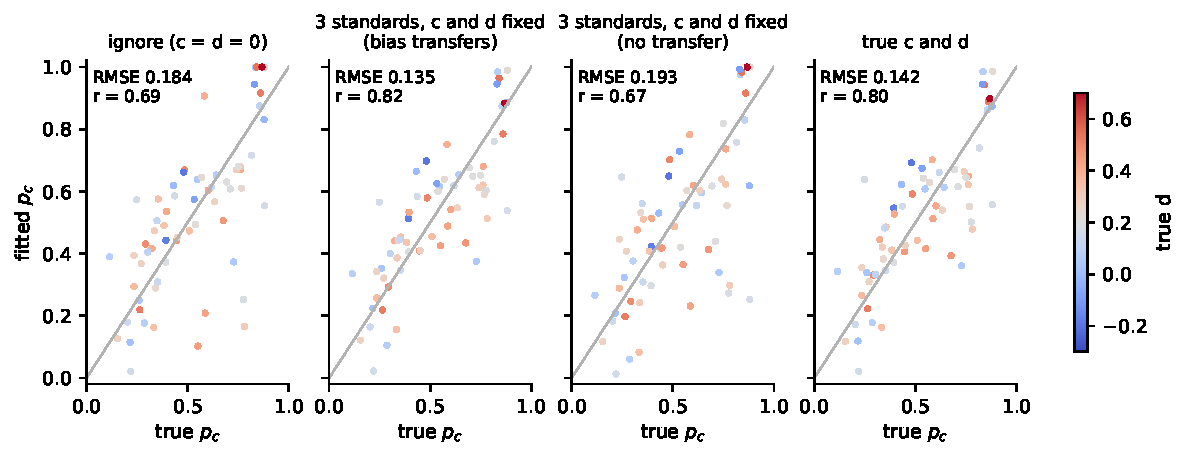
\includegraphics[width=\textwidth]{xm_pc.pdf}
\caption{Fitted against true $\pc$ for the CI participants, coloured by the true $d$.}\label{fig:pc}
\end{figure}

\subsection{How much the bimodal data say about the bias}
Figs.~\ref{fig:size} and~\ref{fig:evidence}.
\begin{itemize}
\item \textbf{Model recovery does not get worse as the bias grows.} With the bias ignored it is 88--93\% for every $d$ above 0.1 and every $c$ above 0.1. The lowest group ($d < 0.1$, 78\%) is equally low with the true bias (76\%), so its errors have other causes.
\item \textbf{The $\pc$ error barely depends on $d$} when the bias is ignored: between $-0.04$ and $+0.04$. The exception is $d > 0.5$, at $+0.08$, which rests on only 4 CI participants.
\item \textbf{Fixing the true bias improves the generating model's fit by a median of about 1 AIC point.} It is more than 2 points for 38\% of participants and more than 10 for 8\%. Negative values occur because $\sigma_A$ and $\sigma_V$ are fixed with error, and the fit without the bias can absorb some of that error.
\end{itemize}

\begin{figure}[H]\centering
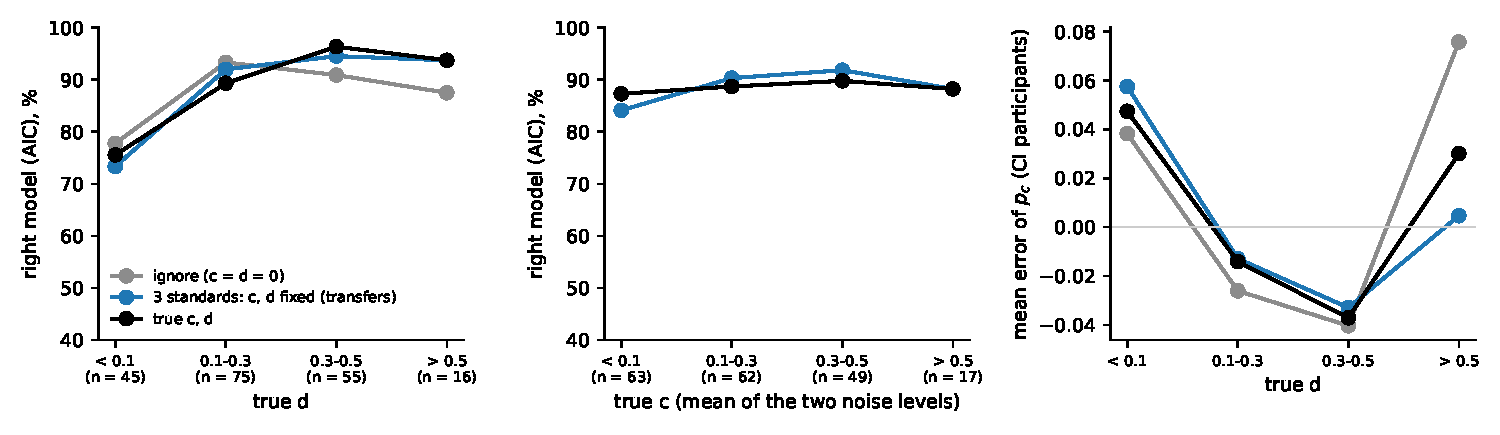
\includegraphics[width=\textwidth]{xm_bias_size.pdf}
\caption{Right model by the true $d$ (left) and the true $c$ (middle), and the mean $\pc$ error by the true $d$ (right).}\label{fig:size}
\end{figure}

\begin{figure}[H]\centering
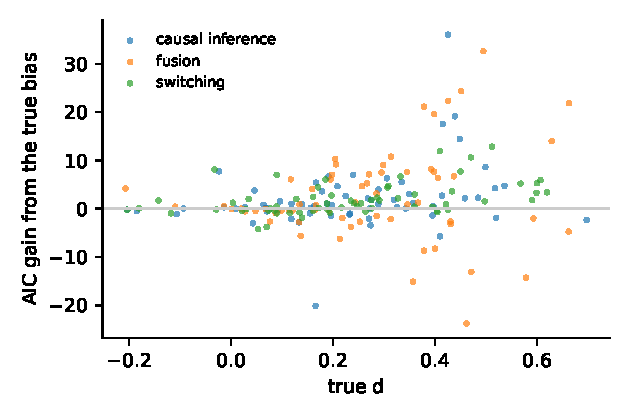
\includegraphics[width=0.5\textwidth]{xm_evidence.pdf}
\caption{AIC of the generating model with the bias ignored minus with the true bias (positive: the true bias fits better), against the true $d$.}\label{fig:evidence}
\end{figure}

\section{v1 real data}\label{sec:v1}
From \texttt{v1\_bias\_fits.py}: 11 participants, about 2,060 trials each, with the physical visual durations (nominal + VisualPSE). v1 measured $c$ at 500\,ms only, so this corresponds to the ``500\,ms block'' option.

\begin{table}[H]\centering\small
\begin{tabular}{lcccccc}
\toprule
 & \multicolumn{2}{c}{same winning model} & \multicolumn{2}{c}{summed AIC change} & \multicolumn{2}{c}{largest $\pc$ change} \\
$\sigma_A$ & $c$ fixed & $c$ fixed, $d$ free & $c$ fixed & $c$ fixed, $d$ free & $c$ fixed & $c$ fixed, $d$ free \\
\midrule
tied to the unimodal block & 9/11 & 9/11 & $-10$ & $-46$ & 0.10 & 0.20 \\
free & 5/11 & 5/11 & $-8$ & $-36$ & 0.45 & 0.55 \\
\bottomrule
\end{tabular}
\caption{v1: fits with $c$ fixed at each participant's cross-modal value, compared with $c = d = 0$. Negative AIC change means a better fit, summed over 11 participants.}
\end{table}

As the simulation predicts:
\begin{itemize}
\item With $\sigma_A$ tied, as in the planned joint fit, the measured $c$ changes little: 9 of 11 winners stay the same, and the AIC improves by about 1 point per participant.
\item With $\sigma_A$ free, the winner is unstable: fixing $c$ changes it for 6 of 11 and $\pc$ by up to 0.45. With few constraints, small changes to the model move v1's model comparison, as expected from its 7-conflict design.
\item These fits use the unimodal $\sigma$ divided by $\sqrt 2$ (measurement noise), as the article does. The version sent earlier on 30 October did not divide, so its $\sigma$s were 41\% too large; this table replaces it.
\end{itemize}

\section{Cost}
\begin{center}\small
\begin{tabular}{lccl}
\toprule
option & trials & time & what it buys \\
\midrule
ignore the bias & 0 & 0 & the same model recovery as the true bias \\
500\,ms block & 400 & about 25\,min & nothing measurable \\
3 standards (300, 500, 800\,ms) & 744 & about 40--45\,min & $\pc$ RMSE 0.18 $\to$ 0.14, if the bias transfers \\
\bottomrule
\end{tabular}
\end{center}
Times are from the lab: 388-trial 500\,ms blocks took 25--28\,min (P101, P104), and P102's 732-trial three-standard session took 38\,min. With the current blocks (216 + 340 + 170 + 2 $\times$ 992 trials, about 2\,h\,15 to 2\,h\,45 of trials), the three-standard block would add a quarter to a third to the total time.

\section{Limits of this simulation}
\begin{itemize}
\item \textbf{Order is left out.} The models and the simulated observers treat test-first and test-second trials alike. The real data show a strong order asymmetry in loud noise (\texttt{bias\_report.pdf}, the section on presentation order). The simulation shows what the bias does if the models are otherwise right; it says nothing about the order effect.
\item \textbf{The bias acts in both intervals in the same way,} as $\ln \hat v = \ln v - c - d \ln(v/0.5)$. A bias that differs between the standard (which carries the conflict) and the test would act differently.
\item \textbf{191 participants.} 600 were planned. The paired differences are precise to about $\pm$2--5 points, enough for the conclusions above but not to resolve differences of 1--2 points.
\item \textbf{The unimodal $\sigma$s are known with a log error of 0.2,} as from 150 + 20 QUEST+ trials. Order-dependent $\sigma_A$ would make them less useful than this.
\end{itemize}

\section*{Files}
\sloppy
In \texttt{av\_dur\_experiment\_v2/analysis/overnight\_sims/}:
\begin{itemize}
\item \texttt{crossmodal\_baseline.py}: the simulation. It is resumable: another run adds participants to \texttt{results/crossmodal\_baseline.json}.
\item \texttt{crossmodal\_analyse.py}: the tables, in \texttt{results/crossmodal\_analyse.txt}; the figures, \texttt{report/xm\_*.pdf}; and the numbers, \texttt{report/xm\_numbers.json}.
\item \texttt{v1\_bias\_fits.py}: the v1 fits, in \texttt{results/v1\_bias\_fits.json}.
\end{itemize}

\end{document}
